\documentclass[aspectratio=169,11pt]{beamer}

\usepackage{fontspec}
\usepackage{polyglossia}
\setmainlanguage{czech}

\usepackage{graphicx}
\usepackage{listings}
\usepackage{xcolor}
\usepackage{hyperref}

% Typography & Colors
\setsansfont{DejaVu Sans}
\setmonofont{DejaVu Sans Mono}

\definecolor{vasulkabg}{RGB}{18, 22, 28}
\definecolor{vasulkatxt}{RGB}{230, 235, 245}
\definecolor{vasulkaamber}{RGB}{245, 158, 11}
\definecolor{vasulkared}{RGB}{239, 68, 68}
\definecolor{vasulkagreen}{RGB}{16, 185, 129}
\definecolor{vasulkacard}{RGB}{28, 34, 44}

\setbeamercolor{background canvas}{bg=vasulkabg}
\setbeamercolor{normal text}{fg=vasulkatxt}
\setbeamercolor{title}{fg=vasulkaamber}
\setbeamercolor{subtitle}{fg=vasulkatxt}
\setbeamercolor{frametitle}{fg=vasulkaamber,bg=vasulkabg}
\setbeamercolor{structure}{fg=vasulkaamber}
\setbeamercolor{block title}{fg=vasulkabg,bg=vasulkaamber}
\setbeamercolor{block body}{fg=vasulkatxt,bg=vasulkacard}

\setbeamertemplate{navigation symbols}{}
\setbeamertemplate{footline}{
  \leavevmode%
  \hbox{%
  \begin{beamercolorbox}[wd=\paperwidth,ht=3ex,dp=1.5ex,leftskip=2ex,rightskip=2ex]{background canvas}%
    \textcolor{gray}{\small Friendly Fire: Mediální archeologie \& Resuscitace} \hfill
    \textcolor{vasulkaamber}{\small \insertframenumber{} / \inserttotalframenumber}
  \end{beamercolorbox}%
  }%
  \vskip0pt%
}

\lstset{
  backgroundcolor=\color{vasulkacard},
  basicstyle=\ttfamily\footnotesize\color{vasulkatxt},
  keywordstyle=\color{vasulkaamber}\bfseries,
  commentstyle=\color{gray},
  stringstyle=\color{vasulkagreen},
  frame=single,
  rulecolor=\color{gray},
  breaklines=true,
  showstringspaces=false
}

\title{\textbf{FRIENDLY FIRE}}
\subtitle{Mediální archeologie a resuscitace díla Woodyho Vašulky}
\author{\textbf{Kryštof Pešek (kof)}}
\institute{Santa Fe (léto 2016) $\rightarrow$ Špilberk Brno (podzim 2016)}
\date{Listopad 2026}

\begin{document}

% Slide 1: Title
\begin{frame}
  \titlepage
  \begin{center}
    \small\textcolor{gray}{--τέχνη \& kof}
  \end{center}
\end{frame}

% Slide 2: Prologue
\begin{frame}{I. Předpolí: Krédo mediální archeologie}
  \begin{block}{Zápis z terénního deníku (Santa Fe, 23. 7. 2016)}
    \textit{„Neznám mnoho palčivějších pocitů než představa jakkoli nepřekonatelné výzvy, která je pro svoji domnělou nepřekonatelnost odmítnuta...\\
    \textbf{Dílo neexistuje, nemá-li kontext.}“}
  \end{block}
  \vspace{0.5cm}
  \begin{columns}
    \begin{column}{0.48\textwidth}
      \textbf{Muzeum vs. Živý stroj:}
      \begin{itemize}
        \item Digitální díla 90. let umírají v depozitářích jako technologické fosilie.
        \item Kurátoři se bojí spálených relé a mrtvých sběrnic.
      \end{itemize}
    \end{column}
    \begin{column}{0.48\textwidth}
      \textbf{Resuscitace, ne pietní sklo:}
      \begin{itemize}
        \item Cílem nebylo vystavit nefunkční hliníkové torzo.
        \item Cílem bylo \textbf{obnovit kinetickou a sonickou choreografii} v původním rytmu autorů.
      \end{itemize}
    \end{column}
  \end{columns}
\end{frame}

% Slide 3: The Brotherhood
\begin{frame}{I. Kontext díla: Cyklus The Brotherhood (1996--1998)}
  \begin{columns}
    \begin{column}{0.55\textwidth}
      Woody Vašulka v 90. letech přechází od video syntézy k \textbf{dekonstrukci válečných technologií}:
      \begin{itemize}
        \item Šest mechanicko-optických interaktivních stolů.
        \item Vojenský vyřazený materiál z Los Alamos a Sandia.
        \item \textbf{Table \#3: Friendly Fire} – zkoumání fenoménu střelby do vlastních řad, kdy technika obrací destrukci proti svým tvůrcům.
        \item Světová premiéra na festivalu ICC v Tokiu (1998).
      \end{itemize}
    \end{column}
    \begin{column}{0.42\textwidth}
      \centering
      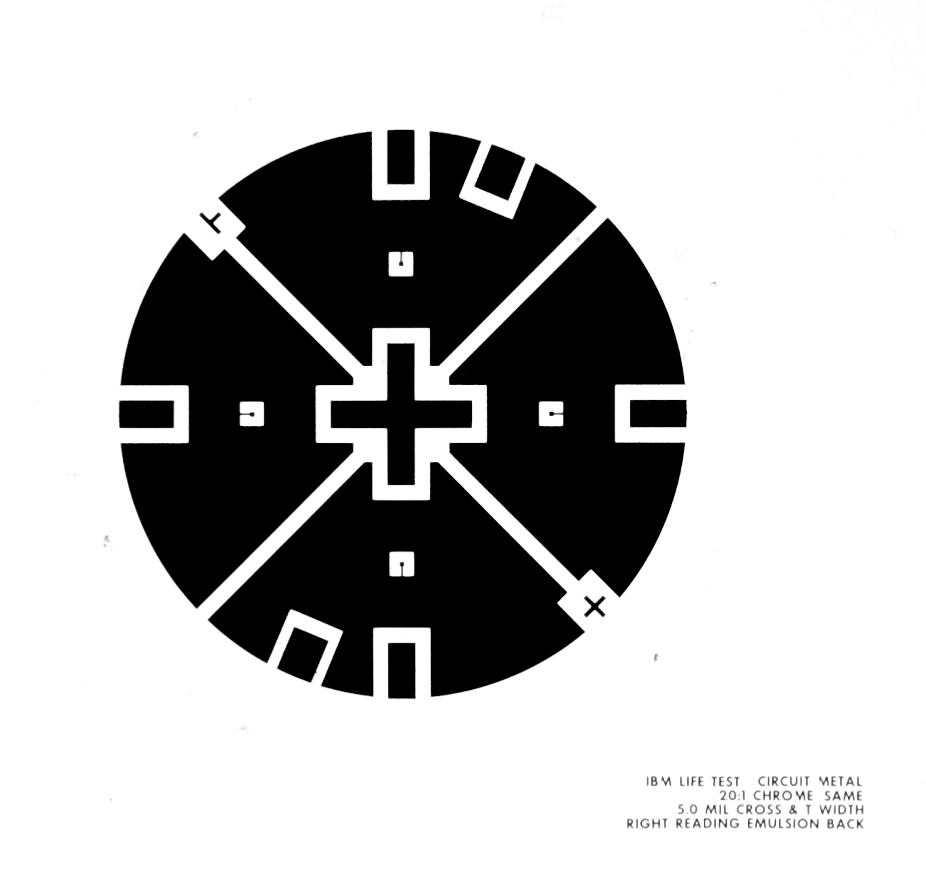
\includegraphics[width=\textwidth]{assets/FF.png}
      \vspace{0.2cm}
      \scriptsize\textcolor{gray}{Woody Vašulka: Table \#3 (Friendly Fire)}
    \end{column}
  \end{columns}
\end{frame}

% Slide 4: Anatomy
\begin{frame}{I. Anatomie Table \#3: Hybridní architektura 90. let}
  \begin{columns}
    \begin{column}{0.32\textwidth}
      \textbf{Pneumatika \& Tělo:}
      \begin{itemize}
        \item Letecký hliník, ocelový rám.
        \item Tlakové vzduchové písty.
        \item 3 padací translucentní clony.
        \item Polopropustná zrcadla.
      \end{itemize}
    \end{column}
    \begin{column}{0.32\textwidth}
      \textbf{Optika \& Obraz:}
      \begin{itemize}
        \item Pioneer LaserDisc přehrávač.
        \item Kodak Carousel 35mm diaprojektor.
        \item SGI IRIX O2 workstation.
        \item Zadní optická projekce.
      \end{itemize}
    \end{column}
    \begin{column}{0.32\textwidth}
      \textbf{Řízení \& Senzory:}
      \begin{itemize}
        \item Intel i386 PC s Linuxem (1997).
        \item Průmyslová relé Opto 22 (LPT).
        \item Roland MIDI pad pro diváka.
        \item Démoni UNICOM v jazyce C.
      \end{itemize}
    \end{column}
  \end{columns}
  \vspace{0.5cm}
  \centering\textcolor{vasulkaamber}{\textbf{Výzva: Každý subsystém vyžadoval jiné napětí, jiný protokol a jinou logiku.}}
\end{frame}

% Slide 5: 18 years
\begin{frame}{I. 18 let hibernace (1998 $\rightarrow$ 2016)}
  \begin{columns}
    \begin{column}{0.5\textwidth}
      Po výstavě v Tokiu v roce 1998 byl stůl rozložen na součástky a uložen v bednách:
      \begin{itemize}
        \item LaserDisc přehrávač zničen, disky nečitelné či ztracené.
        \item Průmyslová deska Opto 22 shořela při testech.
        \item Pneumatické ventily zatuhlé pouštním prachem.
        \item Dokumentace existovala jen v útržcích poznámek.
      \end{itemize}
      \vspace{0.3cm}
      \textbf{Verdikt kurátorů v roce 2015:} \textit{„Nelze zprovoznit, chybí LaserDisc a elektronika.“}
    \end{column}
    \begin{column}{0.45\textwidth}
      \begin{block}{Trojitá smrt mediálního díla}
        \textbf{1. Hardwarová smrt:}\\
        Mechanická relé, optické disky, sběrnice ISA.\\
        \vspace{0.2cm}
        \textbf{2. Softwarová smrt:}\\
        Jádro Linux 2.0.x, binárky SGI IRIX MIPS.\\
        \vspace{0.2cm}
        \textbf{3. Ztráta kontextu:}\\
        Chybějící partitura časování a rytmu pístů.
      \end{block}
    \end{column}
  \end{columns}
\end{frame}

% Slide 6: Santa Fe Mission
\begin{frame}{II. Expedice Santa Fe (Červenec 2016)}
  \begin{columns}
    \begin{column}{0.55\textwidth}
      \textbf{Výsadek v poušti:}
      \begin{itemize}
        \item Telefonát od Jennifer Helia DeFelice (FaVU VUT) zprostředkovaný Milošem Vojtěchovským.
        \item Woody potřeboval někoho, kdo stůl znovu složí a vdechne mu život.
        \item 14 dní v horku Nového Mexika na nalezení, identifikaci a resuscitaci.
        \item Desítky neoznačených beden obsahujících díly ze všech šesti stolů Brotherhoodu.
      \end{itemize}
    \end{column}
    \begin{column}{0.42\textwidth}
      \centering
      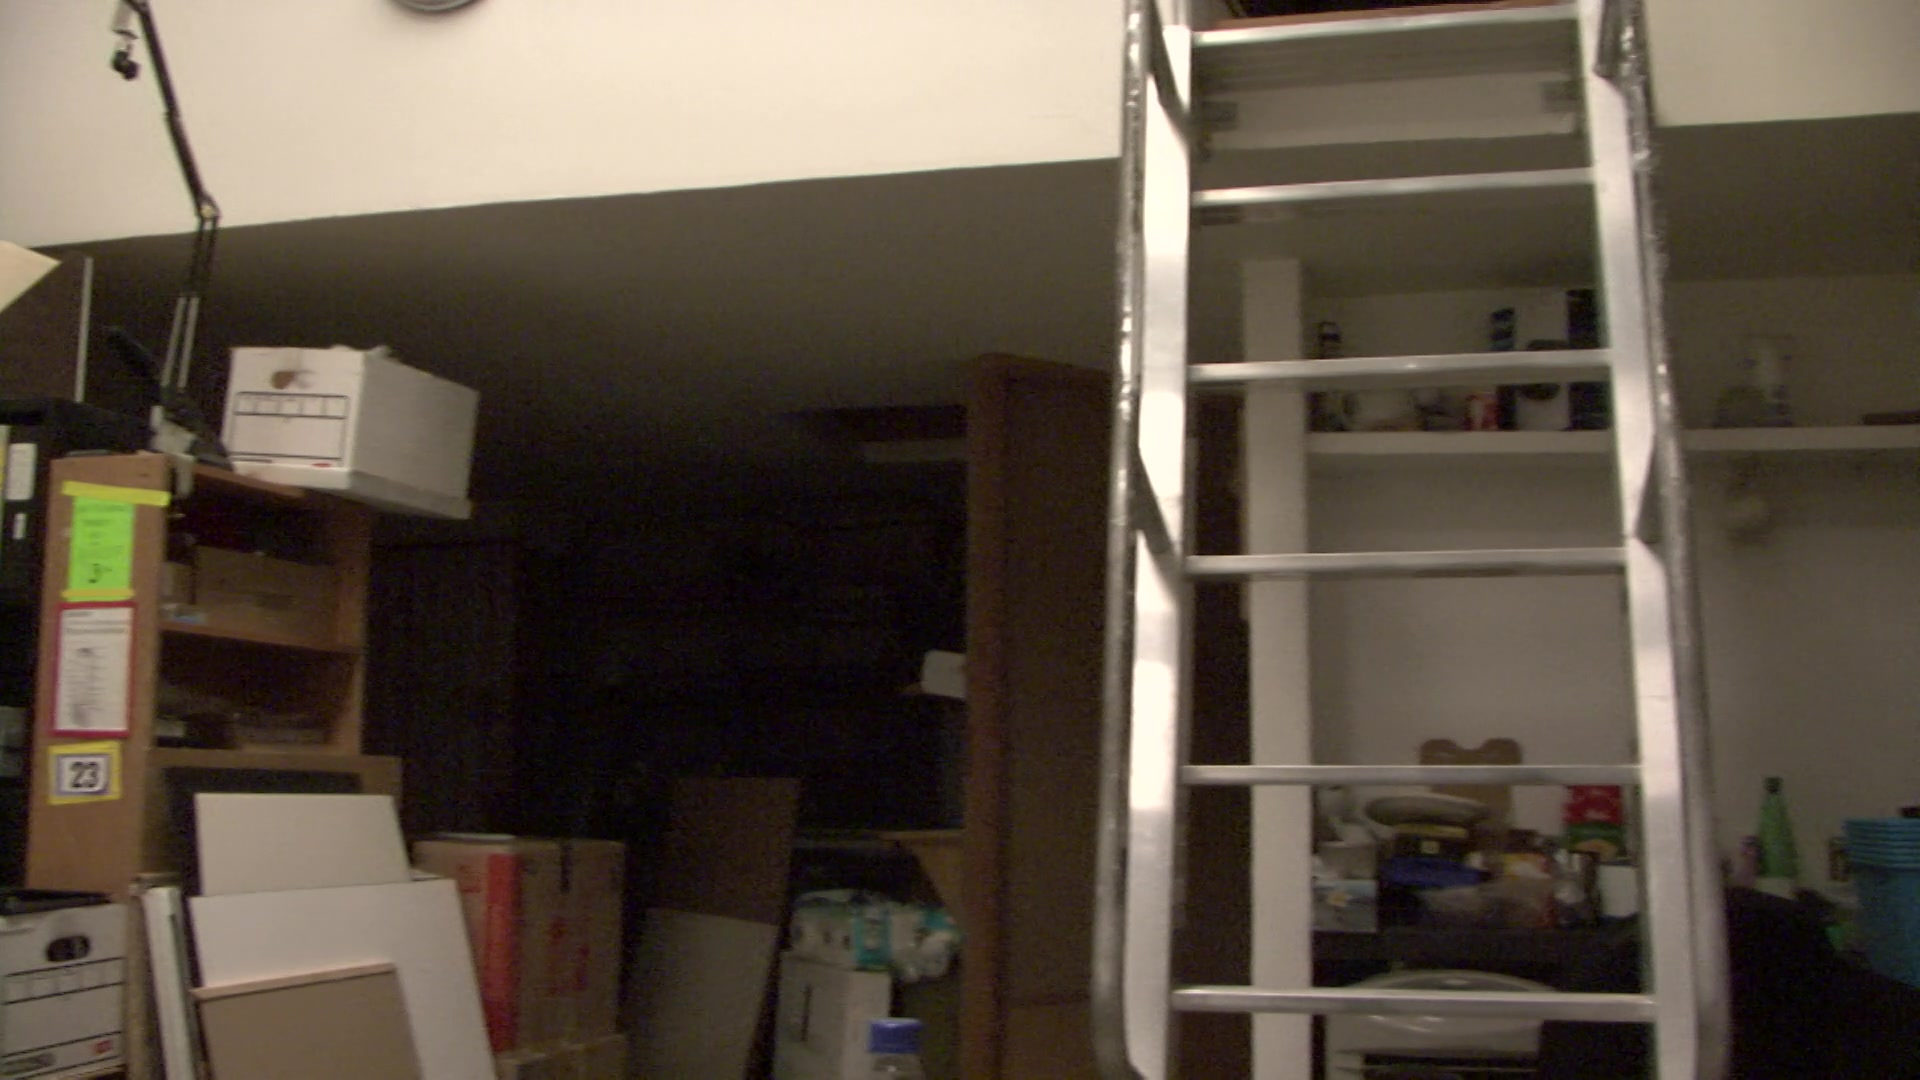
\includegraphics[width=\textwidth]{assets/frame_00.jpg}
      \vspace{0.2cm}
      \scriptsize\textcolor{gray}{Sklad v Santa Fe: Rozpad a chaos součástek}
    \end{column}
  \end{columns}
\end{frame}

% Slide 7: Three Sacred Locations
\begin{frame}{II. Topografie pátrání v Santa Fe}
  \begin{columns}
    \begin{column}{0.32\textwidth}
      \begin{block}{1. Rodeo Road}
        \textbf{Pronajatý sklad:}\\
        Hliníkové profily, bedny z Tokia 1998, původní plotnový disk i386, písty a pneumatické hadice.
      \end{block}
    \end{column}
    \begin{column}{0.32\textwidth}
      \begin{block}{2. Ruffina Street}
        \textbf{Tovární hala:}\\
        Dočasná montážní dílna, translucentní plátna, kompresor, oživování pístů a noční ladění kódu.
      \end{block}
    \end{column}
    \begin{column}{0.32\textwidth}
      \begin{block}{3. Agua Fria Road}
        \textbf{Dům Vašulkových:}\\
        Archiv originálních magnetických pásů, NTSC DV kazety, optika Carouselu, vzpomínky u večeře.
      \end{block}
    \end{column}
  \end{columns}
  \vspace{0.5cm}
  \centering\textit{„Každý den začínal kávou na Agua Fria a končil v noci na Ruffina Street syčením vzduchu.“}
\end{frame}

% Slide 8: Steina
\begin{frame}{II. Steina Vašulková: Živý lidský kompas}
  \begin{columns}
    \begin{column}{0.55\textwidth}
      Ačkoliv Steina tvrdila, že Friendly Fire je čistě Woodyho záležitost, její přítomnost byla rozhodující:
      \begin{itemize}
        \item \textbf{Lidský index:} Přesně věděla, ve které bedně leží zrcadla a kde hledat kabelové svazky.
        \item \textbf{Pracovní motor:} Udržovala disciplínu, stravu a klid uprostřed technického chaosu.
        \item \textbf{První kritické ucho:} Okamžitě odhalila, co v projekci chybí a co je technicky přebujelé.
      \end{itemize}
    \end{column}
    \begin{column}{0.42\textwidth}
      \centering
      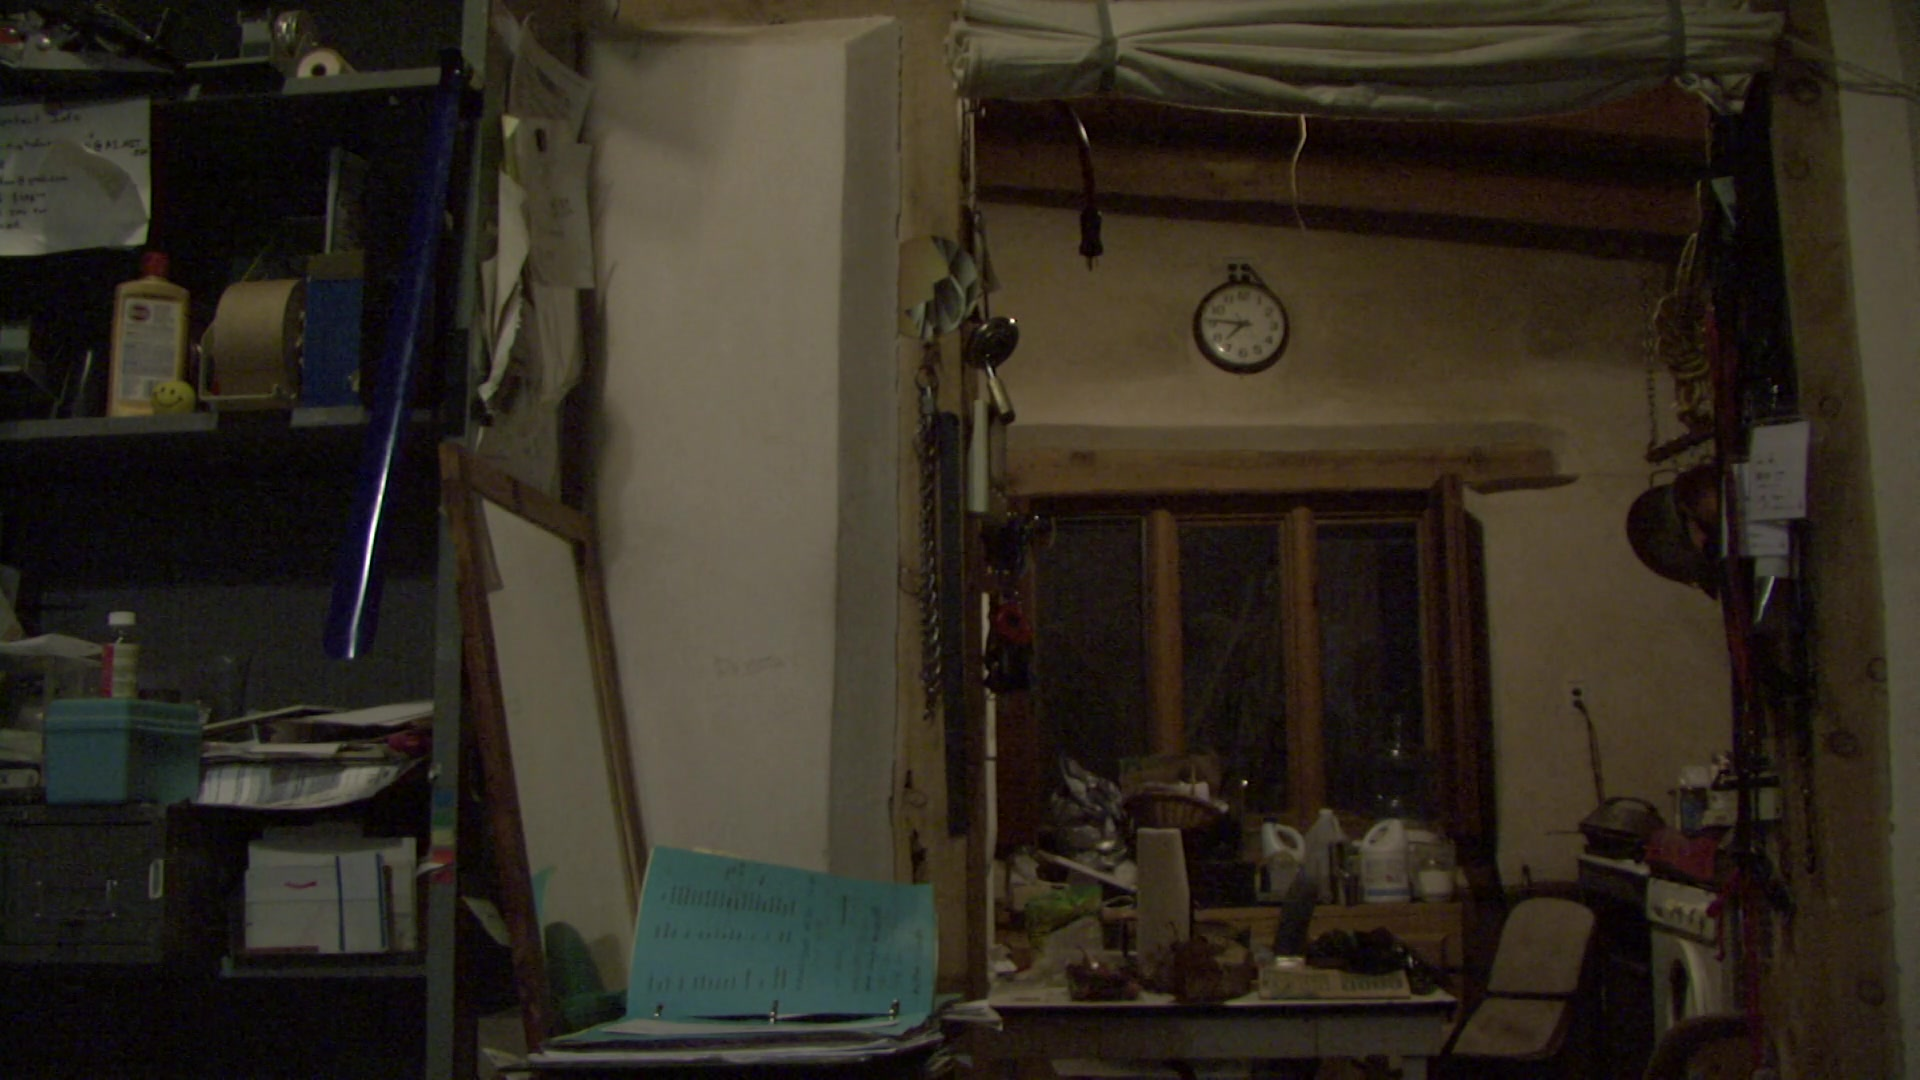
\includegraphics[width=\textwidth]{assets/frame_05.jpg}
      \vspace{0.2cm}
      \scriptsize\textcolor{gray}{Revize optiky a pláten na Ruffina Street}
    \end{column}
  \end{columns}
\end{frame}

% Slide 9: Digital Forensic
\begin{frame}[fragile]{III. Forenzní archeologie: Původní disk z roku 1998}
  \begin{columns}
    \begin{column}{0.5\textwidth}
      Na dně bedny se zdroji nalezen originální plotnový disk PC (Intel i386):
      \begin{itemize}
        \item Připojen přes USB-IDE – disk se bezchybně roztočil!
        \item Bitová kopie disku vytvořena přes \texttt{ddrescue}.
        \item Nalezena netknutá instalace Linuxu z let 1997/1998.
        \item Nalezeny zdrojové kódy démonů v C (\texttt{actor1.c}, \texttt{optodd.c}, \texttt{mididd.c}).
      \end{itemize}
    \end{column}
    \begin{column}{0.48\textwidth}
\begin{lstlisting}[language=bash,caption=Forenzní nález v adresáři]
/home/woody/
|-- actor1.c     # Interpret choreografie
|-- optodd.c     # Driver Opto 22
|-- mididd.c     # Driver MIDI padu
|-- usc/         # Socket Commander
`-- minicom/
    `-- PITT.TXT # Partitura z 8. 3. 1997!
\end{lstlisting}
    \end{column}
  \end{columns}
\end{frame}

% Slide 10: QEMU Emulation
\begin{frame}[fragile]{III. Emulace v QEMU: Oživení systému 1998}
  \textbf{Virtualizace jako most přes propast 18 let:}\\
  Místo shánění základní desky z roku 1997 byl obraz spuštěn ve virtuálním stroji \textbf{QEMU}:
  \vspace{0.2cm}
\begin{lstlisting}[language=bash]
qemu-system-i386 -hda friendlyfire_1998.img -m 64 -serial pty -parallel /dev/parport0
\end{lstlisting}
  \vspace{0.3cm}
  \begin{columns}
    \begin{column}{0.48\textwidth}
      \textbf{Záchrana logiky:}
      \begin{itemize}
        \item Virtuální stroj nabootoval a spustil démony.
        \item Zachráněny přesné časové konstanty a čekací cykly bez nutnosti odhadování.
      \end{itemize}
    \end{column}
    \begin{column}{0.48\textwidth}
      \textbf{Architektonické zjištění:}
      \begin{itemize}
        \item Odhalena modulární UNIXová architektura \textbf{UNICOM} (Russell Gritzo \& Bruce Hamilton).
      \end{itemize}
    \end{column}
  \end{columns}
\end{frame}

% Slide 11: UNICOM Architecture
\begin{frame}{III. Architektura UNICOM (1997)}
  \begin{columns}
    \begin{column}{0.5\textwidth}
      \textbf{Sada spolupracujících démonů:}
      \begin{itemize}
        \item \textbf{\texttt{actor1}:} Interpret scénáře a časování.
        \item \textbf{\texttt{optodd}:} Řízení relé Opto 22 přes \texttt{/dev/lp1}.
        \item \textbf{\texttt{mididd}:} Čtení úderů Roland padu z \texttt{/dev/cua0}.
        \item \textbf{\texttt{picdd}:} Ovladač krokových motorů.
        \item \textbf{\texttt{usc}:} Síťové sockety propojující PC se stanicí SGI O2.
      \end{itemize}
    \end{column}
    \begin{column}{0.48\textwidth}
      \centering
      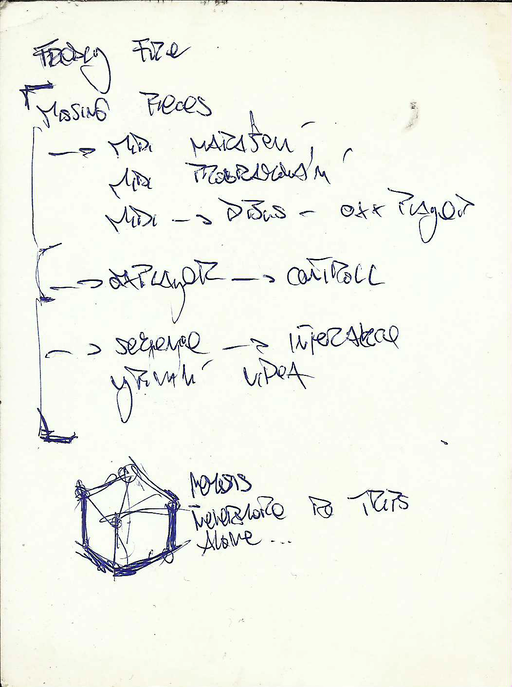
\includegraphics[height=0.68\textheight,width=\textwidth,keepaspectratio]{assets/friendly_fire_16.png}
      \vspace{0.2cm}
      \scriptsize\textcolor{gray}{Blokové schéma toku zpráv UNICOM}
    \end{column}
  \end{columns}
\end{frame}

% Slide 12: PITT.TXT Rosetta Stone
\begin{frame}[fragile]{III. Rozetská deska: PITT.TXT (8. března 1997)}
  V adresáři Minicomu nalezen soubor \texttt{PITT.TXT} – přesný log komunikace s LaserDiskem a relé:
  \vspace{0.2cm}
  \begin{columns}
    \begin{column}{0.48\textwidth}
\begin{lstlisting}[language=bash]
# PITT.TXT (úryvek z 8. 3. 1997)
d08 for 1        # Posun diaprojektoru
5se1801pl        # Seek na frame 5 & play
echo -n "\332" > /dev/lp1 # Clona nahoru
wait 12          # Čekej 12 vteřin
echo -n "\300" > /dev/lp1 # Clona dolů
29082sepl        # Skok na frame 29082
\end{lstlisting}
    \end{column}
    \begin{column}{0.48\textwidth}
      \textbf{Dešifrování partitury stolu:}
      \begin{itemize}
        \item Celková smyčka má přesně \textbf{922 sekund} (15 minut 22 vteřin).
        \item Nalezeny přesné body, kdy úder na pad mění větev choreografie.
        \item Nalezena sekvence výměny diapozitivů v Carouselu.
      \end{itemize}
    \end{column}
  \end{columns}
\end{frame}

% Slide 13: Restoration Ethics
\begin{frame}{IV. Restaurátorská etika: Tělo vs. Orgány}
  \begin{block}{Základní restaurátorská doktrína}
    \centering\large\textbf{„Zachovat tělo a senzorickou zkušenost v plné autenticitě; nahradit zaniklé a neudržitelné vnitřní orgány otevřeným, trvanlivým systémem.“}
  \end{block}
  \vspace{0.4cm}
  \begin{columns}
    \begin{column}{0.48\textwidth}
      \textbf{CO ZŮSTALO PŮVODNÍ (100 \%):}
      \begin{itemize}
        \item Hliníkový stůl a optické stolice.
        \item Pneumatické písty a ventily.
        \item Padací clony a zrcadla.
        \item Kodak Carousel 35mm.
        \item Roland MIDI bicí pad.
      \end{itemize}
    \end{column}
    \begin{column}{0.48\textwidth}
      \textbf{CO BYLO RESUSCITOVÁNO:}
      \begin{itemize}
        \item LaserDisc $\rightarrow$ \textbf{Raspberry Pi (H.264)}.
        \item Opto 22 $\rightarrow$ \textbf{Arduino Uno + SSR relé}.
        \item i386 PC $\rightarrow$ \textbf{Moderní Mini-ITX Linux}.
        \item Uzavřený kód $\rightarrow$ \textbf{Open-source na GitHubu}.
      \end{itemize}
    \end{column}
  \end{columns}
\end{frame}

% Slide 14: Opto 22 to Arduino
\begin{frame}[fragile]{IV. Hardwarová náhrada \#1: Opto 22 $\rightarrow$ Arduino + SSR}
  \begin{columns}
    \begin{column}{0.5\textwidth}
      Spálená obří reléová deska Opto 22 byla neopravitelná. Charles Tuttle navrhl kompaktní modul:
      \begin{itemize}
        \item \textbf{Arduino Uno:} Přijímá příkazy přes USB serial (115 200 baudů).
        \item \textbf{Polovodičová relé (SSR):} Tichá, opticky oddělená, nezpůsobují proudové rázy na cívkách pístů.
        \item Vešlo se do původního montážního boxu ve stole.
      \end{itemize}
    \end{column}
    \begin{column}{0.48\textwidth}
\begin{lstlisting}[language=bash,caption=Protokol sériové linky]
# 1997: Zápis na paralelní port
echo -n "\332" > /dev/lp1

# 2016: ASCII maska relé přes USB
echo -n "/1100000" > /dev/ttyACM0
# Okamžitá čitelnost a debugovatelnost!
\end{lstlisting}
    \end{column}
  \end{columns}
\end{frame}

% Slide 15: LaserDisc to RPi
\begin{frame}[fragile]{IV. Hardwarová náhrada \#2: LaserDisc $\rightarrow$ Raspberry Pi}
  \begin{columns}
    \begin{column}{0.5\textwidth}
      Původní analogový LaserDisc přehrávač Pioneer byl nenávratně ztracen:
      \begin{itemize}
        \item V archivu na Agua Fria nalezen \textbf{originální master na NTSC DV pásku}.
        \item Digitalizace a deinterlace (\texttt{yadif}) do čistého H.264.
        \item Nasazení \textbf{Raspberry Pi} s přehrávačem \texttt{omxplayer} (GPU video).
        \item Řízení seeku v reálném čase přes \textbf{D-Bus rozhraní}.
        \item Reversní chod vyřešen vyrenderováním zpětné stopy videa.
      \end{itemize}
    \end{column}
    \begin{column}{0.48\textwidth}
\begin{lstlisting}[language=bash,caption=D-Bus řízení omxplayeru]
# Skok na pozici v mikrosekundách
dbuscontrol.sh setposition 1801000

# Změna rychlosti / pauza
dbuscontrol.sh pause
# Odezva skoku < 80 ms!
\end{lstlisting}
    \end{column}
  \end{columns}
\end{frame}

% Slide 16: Code Archaeological Diff
\begin{frame}[fragile]{IV. Kódové srovnání v terminálu: 1997 vs. 2016}
  \begin{columns}
    \begin{column}{0.48\textwidth}
\begin{lstlisting}[language=C,caption=1997: UNICOM v jazyce C]
/* actor1.c (1997) */
fd_lp = open("/dev/lp1", O_WRONLY);
write(fd_lp, "\332", 1); /* Písty */

/* Sériový port LaserDisku */
write(fd_ser, "5se1801pl\r", 10);

/* Diaprojektor */
write(fd_ser, "d08 for 1\r", 10);
\end{lstlisting}
    \end{column}
    \begin{column}{0.48\textwidth}
\begin{lstlisting}[language=bash,caption=2016: FriendlyFire Open Source]
# run.sh (2016)
echo -n "/1100000" > /dev/ttyACM0

# Raspberry Pi D-Bus seek
./scripts/dbuscontrol.sh seek 1801000

# Diaprojektor relé 8
echo -n "/00000001" > /dev/ttyACM0
sleep 0.1
echo -n "/00000000" > /dev/ttyACM0
\end{lstlisting}
    \end{column}
  \end{columns}
\end{frame}

% Slide 17: Living Authors
\begin{frame}{V. Zásah žijících autorů: Dílo není fosilie}
  \begin{columns}
    \begin{column}{0.55\textwidth}
      \textbf{Žijící autor mění pravidla hry:}
      \begin{itemize}
        \item Běžná konzervace usiluje o pasivní zakonzervování stavu.
        \item Žijící autoři vidí své dílo po 18 letech novýma očima.
        \item Woody sledoval oživování s inženýrským kánonem vyučeného strojaře – mechanika byla pro něj posvátná.
        \item Steina zasáhla radikálně do zvukové podoby instalace.
      \end{itemize}
    \end{column}
    \begin{column}{0.42\textwidth}
      \centering
      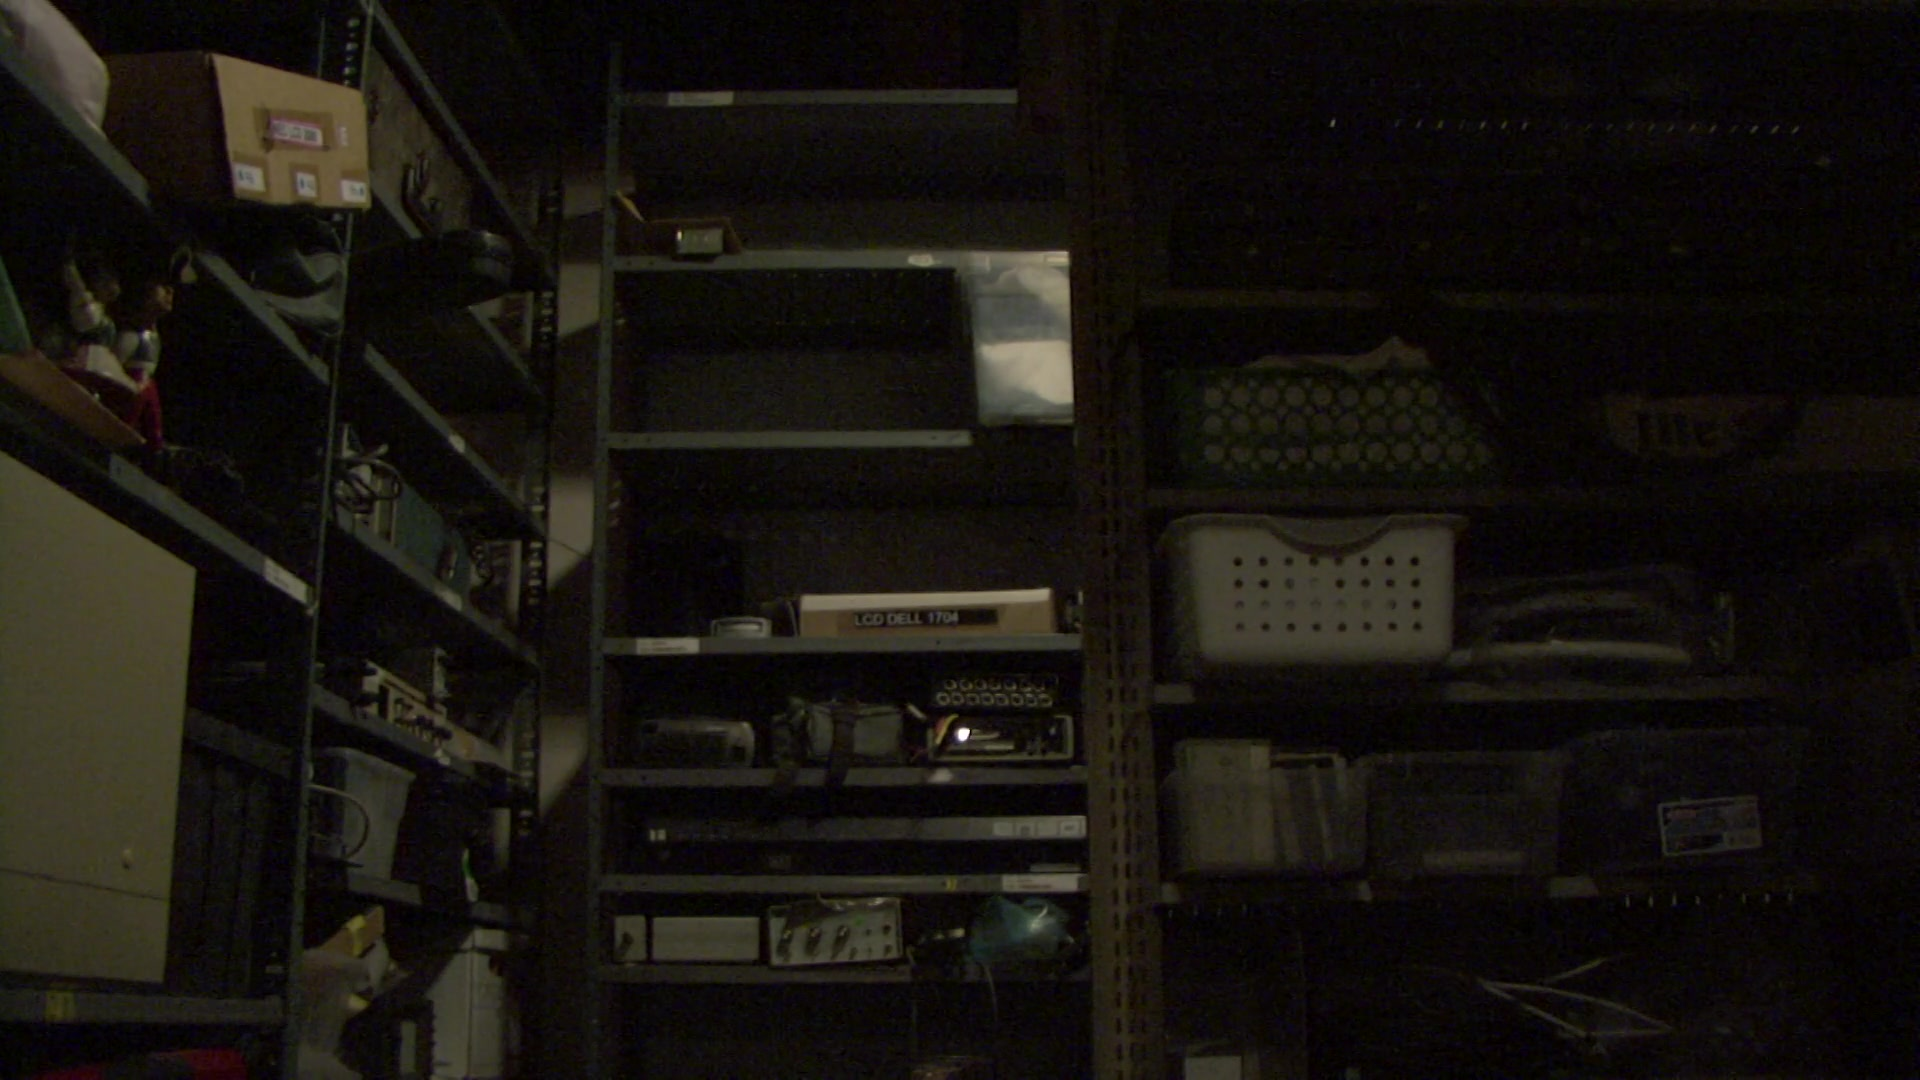
\includegraphics[width=\textwidth]{assets/frame_10.jpg}
      \vspace{0.2cm}
      \scriptsize\textcolor{gray}{Zkoušky pláten v hale na Ruffina Street}
    \end{column}
  \end{columns}
\end{frame}

% Slide 18: Steina audio directive
\begin{frame}{V. Steinino ucho: „Vytáhněte dialogy vojáků!“}
  \begin{columns}
    \begin{column}{0.55\textwidth}
      Když se na Ruffina Street poprvé rozběhla synchronní projekce z Raspberry Pi, Steina poslouchala zvuk v hale a rozhodla:
      \begin{block}{Výrok Steiny Vašulkové}
        \textit{„Ten industriální hluk je moc nahlas. Dialogy operátorů a pilotů jsou utopené. Musíte je vytáhnout do popředí – v těch hlasech je celý smysl Friendly Fire!“}
      \end{block}
      \begin{itemize}
        \item Zvuk byl na místě přemíchán ve prospěch srozumitelnosti řeči.
        \item Autentická vojenská angličtina zůstala bez titulků pro zachování syrovosti.
      \end{itemize}
    \end{column}
    \begin{column}{0.42\textwidth}
      \centering
      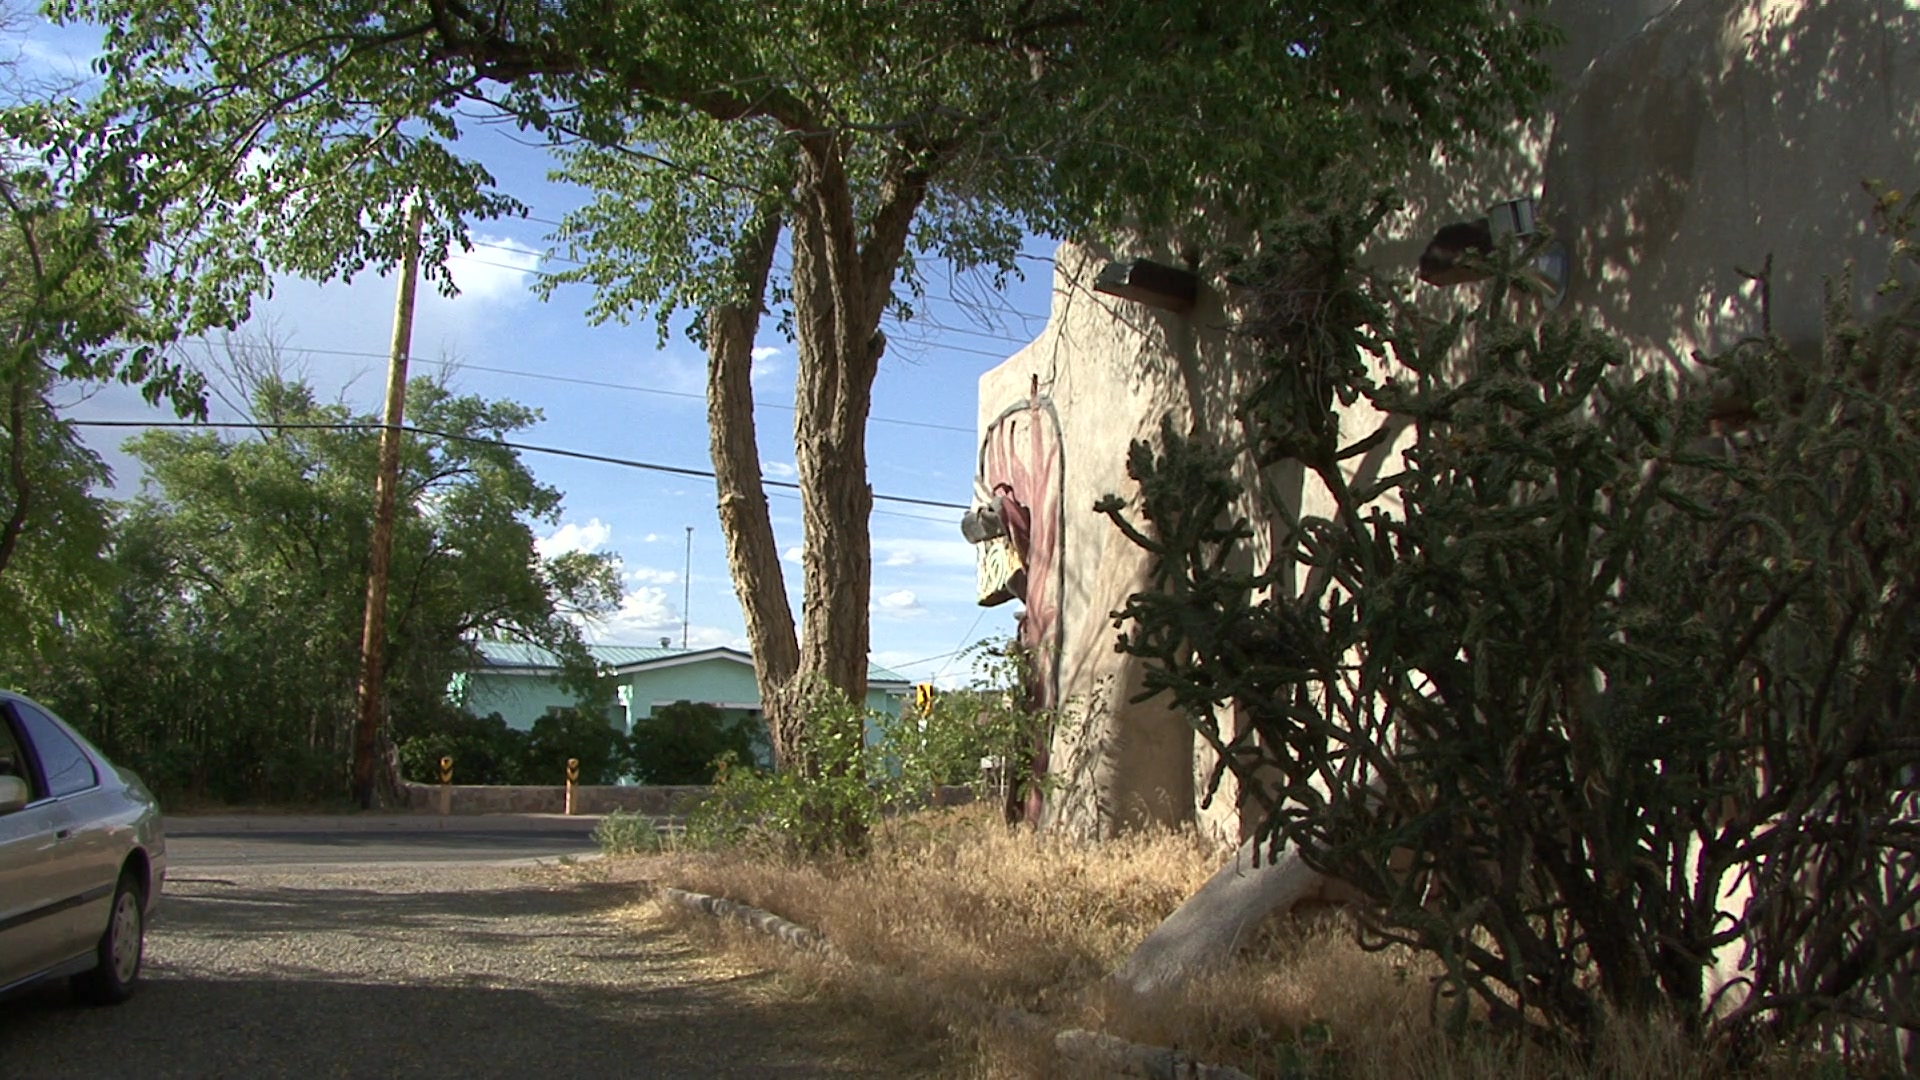
\includegraphics[width=\textwidth]{assets/frame_20.jpg}
      \vspace{0.2cm}
      \scriptsize\textcolor{gray}{Akustické ladění stolu v Santa Fe}
    \end{column}
  \end{columns}
\end{frame}

% Slide 19: Audio Excerpt
\begin{frame}{V. Zvukový archiv: Hlasy Steiny a Woodyho (1. 8. 2016)}
  \begin{block}{Záznam rozhovoru (Agua Fria Road, Zoom H2n)}
    \textbf{Soubor:} \texttt{vasulkas\_brotherhood.opus} (stopáž 38:36)\\
    Nahráno v předvečer sbalení beden pro transport do Evropy.
  \end{block}
  \vspace{0.4cm}
  \textbf{Klíčové myšlenky rozhovoru:}
  \begin{itemize}
    \item Woodyho vzpomínky na brněnskou strojní průmyslovku a posedlost kovovými převody.
    \item Přechod od čistého analogového signálu k fyzickým kinetickým instalacím.
    \item Steina o tom, jak se v 90. letech v Santa Fe prolínaly armádní výprodeje s uměním.
  \end{itemize}
  \vspace{0.3cm}
  \centering\small\textcolor{vasulkaamber}{[Při přednášce pustit 60s ukázku z \texttt{assets/vasulka\_interview\_excerpt.opus}]}
\end{frame}

% Slide 20: Transatlantic Crates
\begin{frame}[fragile]{VI. Návrat do Brna: 67 kg beden přes oceán}
  \begin{columns}
    \begin{column}{0.5\textwidth}
      Otestovaný a zresuscitovaný stůl byl zabalen do tří dřevěných přepravních beden:
      \begin{itemize}
        \item \textbf{Crate \#1 (32 kg):} Hliníková ramena, písty, clony.
        \item \textbf{Crate \#2 (21 kg):} Kodak Carousel, optika, zrcadla.
        \item \textbf{Crate \#3 (14 kg):} Arduino, Raspberry Pi, napájení.
        \item Letecký transport: Albuquerque $\rightarrow$ Chicago $\rightarrow$ Frankfurt $\rightarrow$ Brno.
      \end{itemize}
    \end{column}
    \begin{column}{0.48\textwidth}
\begin{lstlisting}[caption=crates.txt (27. 7. 2016)]
Crate #1: Aluminum frame & pistons
Weight: 32 kg, Dim: 140x60x40 cm
Crate #2: Kodak Carousel & optics
Weight: 21 kg, Dim: 60x50x50 cm
Crate #3: Electronics & controllers
Weight: 14 kg, Dim: 50x40x30 cm
Total weight: 67 kg
Dest: Muzeum mesta Brna, Spilberk
\end{lstlisting}
    \end{column}
  \end{columns}
\end{frame}

% Slide 21: Spilberk Exhibition
\begin{frame}{VI. Výstava na Špilberku (Podzim 2016)}
  \begin{columns}
    \begin{column}{0.5\textwidth}
      Woody Vašulka, rodák z Brna-Židenic, se vrací do rodného města:
      \begin{itemize}
        \item \textbf{Galerijní autonomie:} Stůl musel spolehlivě běžet 8 hodin denně bez dozoru.
        \item Automatický ranní náběh přes \texttt{cron} a \texttt{run.sh}.
        \item Zvednutí clon, spuštění kompresoru, projekce diapozitivů, synchronizace videa.
        \item Večerní bezpečné zaparkování pístů a vypnutí výbojek.
      \end{itemize}
    \end{column}
    \begin{column}{0.48\textwidth}
      \centering
      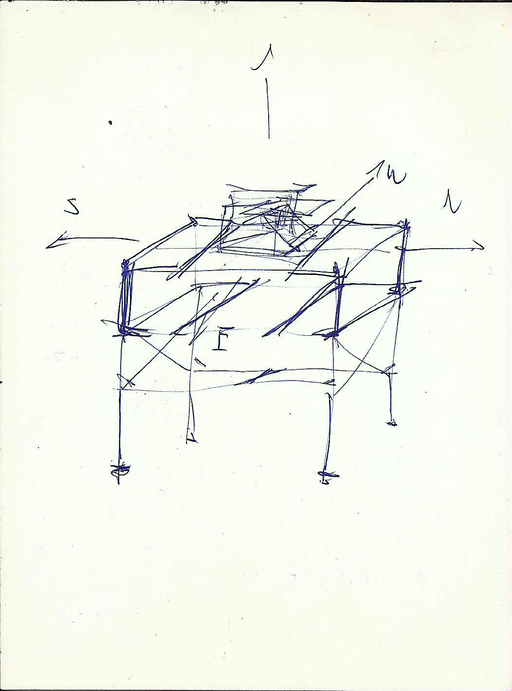
\includegraphics[height=0.68\textheight,width=\textwidth,keepaspectratio]{assets/friendly_fire_table_16.png}
      \vspace{0.2cm}
      \scriptsize\textcolor{gray}{Stavový automat galerijního provozu}
    \end{column}
  \end{columns}
\end{frame}

% Slide 22: Viewer Interaction
\begin{frame}{VI. Divák jako střelec: Roland MIDI Pad}
  \begin{columns}
    \begin{column}{0.55\textwidth}
      \textbf{Kinetická odezva instalace:}
      \begin{itemize}
        \item Před stolem je umístěn bicí pad Roland.
        \item Úder paličkou vyvolává okamžitý výstřel instalace.
        \item Pneumatické písty hlasitě zasyčí a clony spadnou dolů.
        \item Video okamžitě přeskočí na sekvenci výslechu či vojenského útoku.
        \item Carousel cvakne a promítne nový terč na kouřové zrcadlo.
      \end{itemize}
      \vspace{0.3cm}
      \textbf{Divák není pasivní divák, ale operátor zbraně.}
    \end{column}
    \begin{column}{0.42\textwidth}
      \centering
      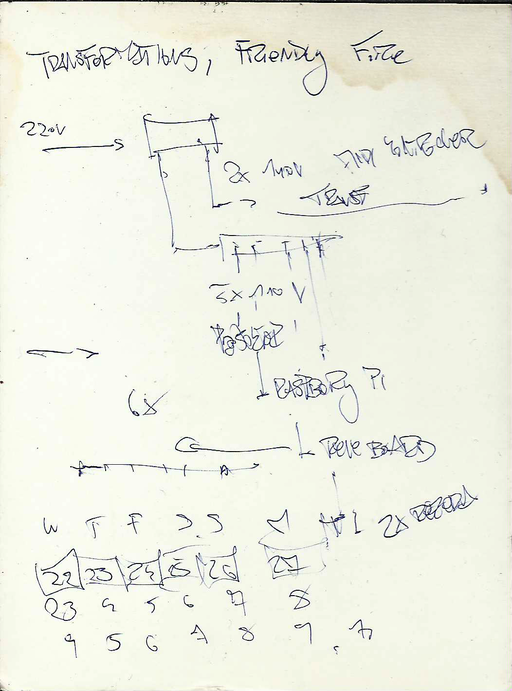
\includegraphics[height=0.68\textheight,width=\textwidth,keepaspectratio]{assets/friendly_fire_transformations_16.png}
      \vspace{0.2cm}
      \scriptsize\textcolor{gray}{Transformační matice reakcí stolu na úder}
    \end{column}
  \end{columns}
\end{frame}

% Slide 23: Lessons Learned
\begin{frame}{VII. Závěry pro mediální archeologii}
  \begin{columns}
    \begin{column}{0.32\textwidth}
      \begin{block}{1. Otevřenost je věčnost}
        Proprietární černé skříňky umírají. Pouze \textbf{otevřený hardware (Arduino, RPi)} a \textbf{svobodný kód (C, Bash)} zaručují přežití díla do dalších dekád.
      \end{block}
    \end{column}
    \begin{column}{0.32\textwidth}
      \begin{block}{2. Živý autor v dílně}
        Resuscitace se žijícími autory je \textbf{pokračováním tvůrčího procesu}. Autor má nezadatelné právo korigovat dílo pro novou éru.
      \end{block}
    \end{column}
    \begin{column}{0.32\textwidth}
      \begin{block}{3. Kód jako notový part}
        Nejlepší dokumentací mediálního díla je \textbf{funkční, verzovaný repozitář na gitu}. Kód je samotnou choreografií instalace.
      \end{block}
    \end{column}
  \end{columns}
  \vspace{0.5cm}
  \centering\textit{„Mediální archeologie není věda o mrtvých přístrojích, ale umění znovu probudit dialog člověka se strojem.“}
\end{frame}

% Slide 24: Epilogue & GitHub
\begin{frame}{VIII. Epilog: Veškerý kód je svobodný}
  \begin{columns}
    \begin{column}{0.6\textwidth}
      Kompletní repozitář se zdrojovými kódy, skripty, deníkem i historickými materiály:
      \vspace{0.3cm}
      \begin{center}
        \Large\texttt{\textcolor{vasulkaamber}{github.com/k0f/friendlyfire}}
      \end{center}
      \vspace{0.3cm}
      \begin{itemize}
        \item Zdrojové kódy démonů, Arduino firmware, shell skripty.
        \item Expediční deník \texttt{LOG.md} ze Santa Fe.
        \item Původní kódy z let 1997--1999 (Russell Gritzo, Bruce Hamilton).
        \item Audio interview se Steinou a Woodym Vašulkovými (1. 8. 2016).
      \end{itemize}
    \end{column}
    \begin{column}{0.38\textwidth}
      \begin{block}{Díky za pozornost}
        \centering
        \textbf{Kryštof Pešek (kof)}\\
        \vspace{0.2cm}
        \small Diskuse, dotazy \& sdílení\\
        \vspace{0.4cm}
        \scriptsize\texttt{--téchné \& kof}
      \end{block}
    \end{column}
  \end{columns}
\end{frame}

\end{document}
